\documentclass[a4paper,12pt, notitlepage]{article}
\usepackage[margin=2.5cm]{geometry}
\usepackage{listings}
\usepackage[parfill]{parskip}
\setlength{\parskip}{\baselineskip}%
\setlength{\parindent}{0pt}%
\usepackage{amsmath}
\usepackage{amssymb}
\usepackage{graphicx}
\usepackage[justification=centering]{caption}
\usepackage{epstopdf}
\usepackage[usenames, dvipsnames]{color}
\usepackage{chngcntr}
\usepackage{titling}
%\counterwithout{footnote}{chapter}
\usepackage{float}
%\renewcommand\theContinuedFloat{\alph{ContinuedFloat}}
\newcommand\tab[1][0.05cm]{\hspace*{#1}}

\title{Numerical Assignment}
\author{Mariana Clare}
\date{\today}

\begin{document}
	
\maketitle
\thispagestyle{empty}
\section{Introduction}
This report will seek to solve the one-dimensional lineriased shallow water equations using four different numerical methods: Co-located Explicit, Co-located Implicit, Staggered Explicit and Staggered Implicit. It will also compare the error between these schemes and the analytic solutions for a given initial condition and test the stability and computational cost of these numerical schemes, as well as how physically realistic they are.

The shallow water equations are
\begin{equation}\label{momentumsw}
\frac{\partial \mathbf{u}}{\partial t} + \mathbf{u}\cdot\nabla\mathbf{u} = - 2\Omega \times\mathbf{u} - g\nabla (h + h_{0})
\end{equation}
\begin{equation}\label{masssw}
\frac{\partial h}{\partial t} + \mathbf{u}\cdot\nabla h = - h \nabla \cdot \mathbf{u}
\end{equation}
where $\mathbf{u}$ is the velocity of the flow, $\Omega$ is the angular velocity of the rotating frame of reference, $g$ is the gravitational acceleration constant, $h$ is the depth of the fluid and $h_{0}$ represents the underlying shape that the fluid is flowing over (as defined in \cite{MPE textbook}).

The first equation (\ref{momentumsw}) represents the conservation of momentum and the second equation (\ref{masssw}) represents the conservation of mass.

Following \cite{MPE textbook}, we will focus consider the one-dimensional form of the equations and linearise them about the state $u = 0$ and $h = H$ ie.
\begin{eqnarray}
\mathbf{u} =  & \mathbf{\hat{u}}
 \\   \nonumber
h = &  H + \hat{h} .
\end{eqnarray}
where $H$ is the average fluid depth. We further assume $h_{0}$ is constant and that the frame is not rotating. Dropping the $\hat{}$ notation this gives
\begin{equation}\label{linearisedsw1}
\frac{\partial u}{\partial t} = - g \frac{\partial h}{\partial x}
\end{equation}
\begin{equation}\label{linearisedsw2}
\frac{\partial h}{\partial t} = - H \frac{\partial u}{\partial x}.
\end{equation}
 Note that throughout this report we assume for simplicity that $u$ and $h$ have periodic boundary conditions.

\section{Numerical Methods}\label{numericalmethodssection}

\subsection {Co-located Explicit}
The first numerical method we use to attempt to solve (\ref{linearisedsw1}) and (\ref{linearisedsw2}) is a simple co-located forward-backward in time and centred in space explicit scheme. As in \cite{MPE textbook}, we consider the scheme to be forward in time for $u$ and backward in time for $h$. Co-located (sometimes referred to as A-grid) means we define the velocity and the height at the same location on the meshgrid.

This scheme can be written as 
\begin{equation} \label{FTCSAgrid}
\frac{u_{j}^{(n+1)} - u_{j}^{(n)}}{\Delta t} = -g \frac{h_{j+1}^{(n)} - h_{j-1}^{(n)}}{2\Delta x}
\end{equation}
\begin{equation}\label{BTCSAgrid}
\frac{h_{j}^{(n+1)} - h_{j}^{(n)}}{\Delta t} = -H \frac{u_{j+1}^{(n+1)} - u_{j-1}^{(n+1)}}{2\Delta x}
\end{equation}
where $h_{j}^{(n)} = h(x_{j}, t^{(n)})$, $u_{j}^{(n)} = h(u_{j}, t^{(n)})$, $x_{j} = j\Delta x$ and $t^{(n)} = n\Delta t$. 

We can determine the order of accuracy of this scheme, by using Taylor series. From \cite{MPE textbook}, we know that both the forward in time and centred in space scheme, and the backward in time and centred in space scheme are first order accurate in time and second order accurate in space. Therefore the co-located explicit scheme is also first order accurate in time and second order accurate in space.

In order to find when this scheme is stable, we use a Von-neumann stability analysis. As in \cite{MPE textbook}, we assume that $u$ and $h$ have wave-like solutions with an amplification factor $A$ and wavenumber $k$:
\begin{equation} \label{wavelikeu}
u  =  \mathbb{U}  A^{n} e^{ikj\Delta x}
\end{equation}
\begin{equation} \label{wavelikeh}
h  =  \mathbb{H} A^{n} e^{ikj\Delta x}
\end{equation}
for constant $\mathbb{U}$ and $\mathbb{H}$.

Further if we define the Courant number 
\begin{equation}\label{Courantnumber}
c = \frac{\sqrt{gH}\Delta t}{\Delta x}
\end{equation}

then substituting these solutions into (\ref{FTCSAgrid}) and (\ref{BTCSAgrid}) gives
\begin{equation}
A = 1 - \frac{c^{2}}{2} \sin^{2}(k\Delta x) \pm \frac{ic}{2}\sin(k\Delta x)\sqrt{4 - c^{2}\sin^{2}k\Delta x}.
\end{equation} 
 
Hence as found in \cite{MPE textbook}, when $\lvert c \rvert \leq 2$, $\lvert A \rvert^{2} = 1$ and the scheme is stable, but when $\lvert c \rvert > 2$, the scheme is unstable.
 
We can also find the dispersion relation, because the frequency of the numerical method is 
\begin{equation} \label{frequency}
\omega = \pm \frac{1}{\Delta t} \arctan\bigg(\frac{Im(A)}{Re(A)}\bigg).
\end{equation}
Using the result from \cite{MPE textbook}, 
\begin{equation}
\omega_{n}\Delta x = \pm \frac{2}{c} \sin^{-1} \bigg(\frac{c}{2}\sin(k\Delta x)\bigg),
\end{equation}
assuming $\sqrt{gH} = 1$. The positive branch of this dispersion relation is plotted in Figure \ref{dispersionfigure} and compared with the dispersion relation of the analytical solution. This shows that the analytic solution and numerical solution do not propagate at the same rate. The numerical solution disperses too slowly and in fact for $k = \pi$, the wave is stationary.

Note the dispersion relation of the analytical solution $\omega = k\sqrt{gH}$ is found by substituting the wave-like solutions (\ref{wavelikeu}) and (\ref{wavelikeh}) into (\ref{linearisedsw1}) and (\ref{linearisedsw2}). 

\subsection{Co-located Implicit}
We would like to have a method that was stable for all Courant numbers. Therefore another method we can use is an implicit method on a co-located grid. As in \cite{MPE textbook}, we will consider the backward in time for both $u$ and $h$ and centred in space co-located scheme:
\begin{equation} \label{FTimplicitAgrid1}
\frac{u_{j}^{(n+1)} - u_{j}^{(n)}}{\Delta t} = -g \frac{h_{j+1}^{(n+1)} - h_{j-1}^{(n+1)}}{2\Delta x}
\end{equation}
\begin{equation}\label{FTimplicitAgrid2}
\frac{h_{j}^{(n+1)} - h_{j}^{(n)}}{\Delta t} = -H \frac{u_{j+1}^{(n+1)} - u_{j-1}^{(n+1)}}{2\Delta x}.
\end{equation}

In order to find the values of $h_{j}^{n}$ and $u_{j}^{n}$ at the next time iteration for all $j$, we consider the matrix:

\[
A = \left (
\begin{array}{ccc}
\begin{array}{ccccc}
1 + \frac{c^{2}}{2} & 0 & -\frac{c^{2}}{4} & 0 & 0\\
0& 1 + \frac{c^{2}}{2} & 0 & -\frac{c^{2}}{4} & 0\\
-\frac{c^{2}}{4} & 0& 1 + \frac{c^{2}}{2} & 0 & -\frac{c^{2}}{4}\\
\vdots & & \vdots & & \vdots\\
- \frac{c^{2}}{4} & 0 & 0 & 0 & 0\\
0 & - \frac{c^{2}}{4} & 0 & 0 & 0\\
\end{array}
\begin{array}{c}
\vdots\\ 
\ddots\\
\vdots
\end{array}
\begin{array}{ccccc}
0 & 0 & 0 & - \frac{c^{2}}{4} & 0\\
0 & 0 & 0 & 0 & - \frac{c^{2}}{4}\\
\vdots & & \vdots & & \vdots\\
-\frac{c^{2}}{4}& 0 & 1 + \frac{c^{2}}{2} & 0 & -\frac{c^{2}}{4} \\
0 & -\frac{c^{2}}{4} & 0 & 1 + \frac{c^{2}}{2} & 0\\
0 & 0 & -\frac{c^{2}}{4}& 0 & 1 + \frac{c^{2}}{2}
\end{array}
\end{array}
\right )
\]

where $c$ is the Courant number as before. 

We write the scheme (\ref{FTimplicitAgrid1}) and (\ref{FTimplicitAgrid2}) as a matrix equation $A \mathbf{x} = \mathbf{b}$ where $\forall j \in [0, N-1]$
\begin{eqnarray}
x_{j} & = & h_{j}^{(n+1)}\\
b_{j} & = & h_{j}^{(n)} - \frac{c}{2}\sqrt{\frac{H}{g}}\bigg(u_{j+1}^{(n)} - u_{j-1}^{(n)}\bigg)
\end{eqnarray}
if solving for $h$ and
\begin{eqnarray}
x_{j} & = & u_{j}^{(n+1)}\\
b_{j} & = & u_{j}^{(n)} - \frac{c}{2}\sqrt{\frac{g}{H}}\bigg(h_{j+1}^{(n)} - h_{j-1}^{(n)}\bigg) 
\end{eqnarray}
if solving for $u$.

Furthermore, as we are assuming periodic boundary conditions, $u_{0}^{(n)} = u_{N}^{(n)}$ and $h_{0}^{(n)} = h_{N}^{(n)}$ where $N\Delta x$ is the maximum value of $x$ in the $x$-domain. Hence the matrix $A$ has dimension $N \times N$ and we consider the first row to be $j = 0$. 

We can determine the order of accuracy of this scheme, as before by using Taylor series expansions.  From \cite{MPE textbook}, we know that both the backward in time and centred in space scheme is first order accurate in time and second order accurate in space. Therefore the staggered explicit scheme is also first order accurate in time and second order accurate in space.

In order to find where this method is stable, we use Von-Neumann stability analysis and assume $u$ and $h$ have wave-like solutions (\ref{wavelikeu}) and (\ref{wavelikeh}). Substituting these solutions into (\ref{FTimplicitAgrid1}) and (\ref{FTimplicitAgrid2}) we find
\begin{equation}
A = \frac{1 \pm i c\sin(k\Delta x)}{1 + c^{2}\sin^{2}(k\Delta x)}
\end{equation}
Therefore $\lvert A \rvert ^{2} < 1$ and the scheme is uncondtionally stable (ie. stable for all Courant numbers). 

Using (\ref{frequency}) we can find the dispersion relation
\begin{equation}
\omega_{n} \Delta x = \pm\frac{\Delta x}{\Delta t} \arctan(c\sin(k\Delta x)) = \frac{1}{c}  \arctan(c\sin(k\Delta x))
\end{equation}
assuming $\sqrt{gH} = 1$. The positive branch of this dispersion relation is again plotted in Figure \ref{dispersionfigure}. Again as with the explicit method, the numeric solution disperses too slowly and in fact at $k = \pi$, the wave is stationary. 

\subsection{Staggered Explicit}
Next we seek a scheme which propagates at a speed more similar to the analytic solution. Following \cite{MPE textbook}, we use a staggered grid (sometimes known as a C-grid) instead of a co-located grid. For a staggered grid, we shift $u$ so that it is defined at $x_{j} + \frac{\Delta x}{2}$ and $h$ remains defined at $x_{j}$ (where $x_{j} = j \Delta x$) ie. $u$ and $h$ are defined alternately in space.

As in \cite{MPE textbook}, we take again the forward-backward in time and centred in space scheme where the scheme is forward in $u$ and backward in $h$, but now we use a staggered grid. This gives us the following scheme:

\begin{equation}\label{FTCSCgrid}
\frac{u_{j+ \frac{1}{2}}^{(n+1)} - u_{j + \frac{1}{2}}^{(n)}}{\Delta t} = -g \frac{h_{j+1}^{(n)} - h_{j}^{(n)}}{\Delta x}
\end{equation}

\begin{equation}\label{BTCSCgrid}
\frac{h_{j}^{(n+1)} - h_{j}^{(n)}}{\Delta t} = -H \frac{u_{j+\frac{1}{2}}^{(n+1)} - u_{j-\frac{1}{2}}^{(n+1)}}{\Delta x}
\end{equation}


We can determine the order of accuracy of this scheme on a staggered grid by using the following Taylor series expansions 
\begin{equation}
h_{j + 1}^{(n)} = h_{j}^{(n)} + \Delta x  \frac{\partial h_{j}^{(n)}}{\partial x} + \frac{(\Delta x)^{2}}{2}\frac{\partial^{2} h_{j}^{(n)}}{\partial x^{2}} + \frac{(\Delta x)^{3}}{6}\frac{\partial^{3} h_{j}^{(n)}}{\partial x^{3}} + O((\Delta x)^{4})
\end{equation}
\begin{equation} \label{uj+1/2n}
u_{j \pm \frac{1}{2}}^{(n)} = u_{j}^{(n)} \pm \frac{\Delta x}{2}\frac{\partial u_{j}^{(n)}}{\partial x} + \frac{(\Delta x)^{2}}{8}\frac{\partial^{2}u_{j}^{n}}{\partial x^{2}} + O({(\Delta x)^{3}}.
\end{equation}
\begin{equation} \label{uj+1/2n+1}
u_{j \pm \frac{1}{2}}^{(n + 1)} = u_{j}^{(n)} \pm \frac{\Delta x}{2}\frac{\partial u_{j}^{(n)}}{\partial x} + \Delta t \frac{\partial u_{j}^{(n)}}{\partial t} + \frac{(\Delta x)^{2}}{8}\frac{\partial^{2}u_{j}^{n}}{\partial x^{2}} \pm \frac{\Delta t \Delta x}{2}\frac{\partial^{2} u_{j}^{(n)}}{\partial x \partial t} + \frac{(\Delta t)^{2}}{2} \frac{\partial ^{2} u_{j}^{(n)}}{\partial t ^{2}} + O((\Delta x)^{3}, (\Delta t)^{3})
\end{equation}

Substituting these into (\ref{FTCSCgrid}), we find that 
\begin{equation}
\frac{\partial u_{j}^{(n)}}{\partial t} + O(\Delta t) =  -g \frac{\partial h_{j}^{(n)}}{\partial x} + O((\Delta x)^{2})
\end{equation} 
and therefore the scheme is first order accurate in time and second order accurate in space. (Note the same order of accuracy is obtained by performing the same analysis with equation (\ref{BTCSCgrid})).

In order to find where this method is stable, we use Von-Neumann stability analysis and assume $u$ and $h$ have wave-like solutions (\ref{wavelikeu}) and (\ref{wavelikeh}). Substituting these solutions into (\ref{FTCSCgrid}) and (\ref{BTCSCgrid}) we find
\begin{equation}
A = 1 - 2c^{2}\sin^{2}\bigg(\frac{k\Delta x}{2}\bigg) \pm 2ic\sin\bigg(\frac{k\Delta x}{2}\bigg) \sqrt{1 - c^{2}\sin^{2}(\frac{k\Delta x}{2}\bigg)}
\end{equation}
Therefore if $\lvert c \rvert \leq 1$, this scheme is stable, but if $\lvert c \rvert > 1$ the scheme is unstable.

Using (\ref{frequency}) we can find the dispersion relation
\begin{equation}
	\omega_{n} \Delta x = \pm\frac{2\Delta x}{\Delta t} \arcsin\bigg(c\sin\bigg(\frac{k\Delta x}{2}\bigg)\bigg) = \frac{2}{c} \arcsin\bigg(c\sin\bigg(\frac{k\Delta x}{2}\bigg)\bigg) 
\end{equation}
assuming $\sqrt{gH} = 1$. The positive branch of this dispersion relation is again plotted in Figure \ref{dispersionfigure}. Although this solution is still dispersive we can see from the Figure that $\omega$ of this numeric scheme is much closer to $\omega$ of the analytic solution.

\subsection{Staggered Implicit}
With the staggered explicit method, we again have the problem that the solution is unstable for some Courant numbers. Therefore the final numerical scheme we will look at is the implicit scheme on a staggered grid, as outlined in \cite{implicit}.

The scheme used in \cite{implicit} is the theta-method:
\begin{equation}
\frac{u_{j + \frac{1}{2}}^{(n + 1)} - u_{j + \frac{1}{2}}^{(n)}}{\Delta t} = -\frac{g}{\Delta x} \bigg(\theta (h_{j + 1}^{(n+ 1)} - h_{j}^{(n+ 1)}) + (1 - \theta) (h_{j + 1}^{(n)} - h_{j}^{(n)})\bigg),
\end{equation}
\begin{equation}
\frac{h_{j}^{(n + 1)} - h_{j}^{(n)}}{\Delta t} = -\frac{H}{\Delta x} \bigg(\theta (u_{j + \frac{1}{2}}^{(n+ 1)} - u_{j - \frac{1}{2}}^{(n+ 1)}) + (1 - \theta) (u_{j + \frac{1}{2}}^{(n)} - u_{j - \frac{1}{2}}^{(n)})\bigg).
\end{equation}

In \cite{implicit} it is shown that if we take $\theta = \frac{1}{2}$ the scheme is second order accurate. Therefore we will take $\theta = \frac{1}{2}$ and are using the Crank-Nicholson method centred in space on a staggered grid:

\begin{equation}\label{semiimplicit1}
\frac{u_{j + \frac{1}{2}}^{(n + 1)} - u_{j + \frac{1}{2}}^{(n)}}{\Delta t} = -\frac{g}{2\Delta x} \bigg((h_{j + 1}^{(n+ 1)} - h_{j}^{(n+ 1)}) + (h_{j + 1}^{(n)} - h_{j}^{(n)})\bigg)
\end{equation}
\begin{equation}\label{semiimplicit2}
\frac{h_{j}^{(n + 1)} - h_{j}^{(n)}}{\Delta t} = -\frac{H}{2\Delta x} \bigg((u_{j + \frac{1}{2}}^{(n+ 1)} - u_{j - \frac{1}{2}}^{(n+ 1)}) + (u_{j + \frac{1}{2}}^{(n)} - u_{j - \frac{1}{2}}^{(n)})\bigg)
\end{equation}

In order to find the values of $h_{j}^{n}$ and $u_{j}^{n}$ at the next time iteration for all $j$, we consider the matrix:

\[
A = \left (
\begin{array}{ccc}
\begin{array}{ccc}
1 + \frac{c^{2}}{2} & -\frac{c^{2}}{4} & 0\\
-\frac{c^{2}}{4}& 1 + \frac{c^{2}}{2} & -\frac{c^{2}}{4} \\
\vdots & \vdots & \vdots\\
0 & 0  & 0 \\
- \frac{c^{2}}{4}  & 0  & 0 
\end{array}
\begin{array}{c}
\vdots\\ 
\ddots\\
\vdots
\end{array}
\begin{array}{ccc}
0  & 0  &  - \frac{c^{2}}{4}\\
0  & 0& 0\\
\vdots & \vdots & \vdots\\
-\frac{c^{2}}{4}& 1 + \frac{c^{2}}{2} & -\frac{c^{2}}{4} \\
0 & -\frac{c^{2}}{4} & 1 + \frac{c^{2}}{2}
\end{array}
\end{array}
\right )
\]
where $c$ is the Courant number as before. 

We write the scheme (\ref{semiimplicit1}) and (\ref{semiimplicit2}) as matrix equation $A \mathbf{x} = \mathbf{b}$ where $ \forall j \in [0, N-1]$
\begin{eqnarray}
x_{j} &= & h_{j}^{(n+1)}\\
b_{j} &= & -c\sqrt\frac{g}{H}\bigg(h_{j + 1}^{(n)} - h_{j}^{n}\bigg) + \frac{c^{2}}{4} u_{j + \frac{3}{2}}^{(n)} + \bigg(1 - \frac{c^{2}}{2}\bigg)u_{j + \frac{1}{2}}^{(n)} + \frac{c^{2}}{4} u_{j - \frac{1}{2}}^{(n)}
\end{eqnarray}
if solving for $h$ and
\begin{eqnarray}
x_{j} & =& u_{j+ \frac{1}{2}}^{(n+1)} \\
b_{j} &= &-c\sqrt\frac{H}{g}\bigg(u_{j + \frac{1}{2}}^{(n)} - u_{j - \frac{1}{2}}^{n}\bigg) + \frac{c^{2}}{4} h_{j + 1}^{(n)} + \bigg(1 - \frac{c^{2}}{2}\bigg)h_{j}^{(n)} + \frac{c^{2}}{4} h_{j - 1}^{(n)}
\end{eqnarray}
if solving for $u$.

Furthermore, as we are assuming periodic boundary conditions, $u_{\frac{1}{2}}^{(n)} = u_{N + \frac{1}{2}}^{(n)}$ and $h_{0}^{(n)} = h_{N}^{(n)}$ where $N\Delta x$ is the maximum value of $x$ in the $x$-domain. Hence the matrix $A$ has dimension $N \times N$ and we consider the first row to be $j = 0$.

From \cite{implicit} the scheme is second order accurate in time and second order accurate in space which is better than any of the other schemes we have looked at so far.

As before in order to find where this method is stable, we use Von-Neumann stability analysis and assume $u$ and $h$ have wave-like solutions (\ref{wavelikeu}) and (\ref{wavelikeh}). Substituting these solutions into (\ref{semiimplicit1}) and (\ref{semiimplicit2}) we find:

\begin{equation}
A = \frac{2 - 2c^{2}\sin^{2}(\frac{k\Delta x}{2}) \pm 4ic\sin(\frac{k\Delta x}{2})}{2 + 2 c^{2}\sin^{2}(\frac{k\Delta x}{2})}
\end{equation}

$\lvert A \rvert^{2} = 1$ and therefore the scheme is unconditionally stable (ie. stable for all courant numbers) $\forall k$.

Using (\ref{frequency}) we can find the dispersion relation
\begin{equation}
\omega_{n} \Delta x = \pm\frac{\Delta x}{\Delta t} \arctan\bigg(\frac{2 c \sin(\frac{k\Delta x}{2})}{1 - c^{2} \sin^{2}(\frac{k\Delta x}{2})}\bigg) = \pm\frac{1}{c} \arctan\bigg(\frac{2 c \sin(\frac{k\Delta x}{2})}{1 - c^{2} \sin^{2}(\frac{k\Delta x}{2})}\bigg)
\end{equation}
assuming $\sqrt{gH} = 1$. The positive branch of this dispersion relation is again plotted in Figure \ref{dispersionfigure}. 

As with the previous staggered grid scheme, this solution is still dispersive, but much less so than either of the co-located schemes. The dispersion relation for the implicit staggered scheme diverges more from the analytic solution than the explicit staggered scheme but the difference is very small. 

\begin{figure}[H]
	\begin{center}

	\centering
	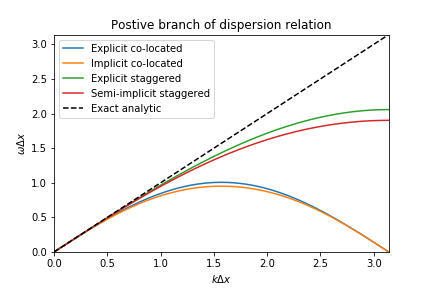
\includegraphics[width=0.6\textwidth]{dispersion_relations.png}
	\caption{Positive branch of dispersion relation $\omega$ for analytic solution and numerical schemes. Note that as in \cite{MPE textbook}, we have used $c=0.4$ and $\sqrt{gH} = 1$.} \label{dispersionfigure}

	\end{center}
\end{figure}

\section{Results}\label{resultssection}
In order to examine the numerical methods outlined in the above section we now conduct a series of tests on a variety of initial conditions. Note for all the follwing results:
\begin{eqnarray}
H & = & 1\\
g & = & 1
\end{eqnarray}
where $H$ is the average fluid depth, $g$ is the gravitational acceleration constant.

\renewcommand\theContinuedFloat{\alph{ContinuedFloat}}
\begin{figure}[H]
	\begin{minipage}{.5\textwidth}
	\ContinuedFloat*
	%\centering
	\captionsetup{width=0.9\textwidth}
	\captionsetup{justification=centering}
	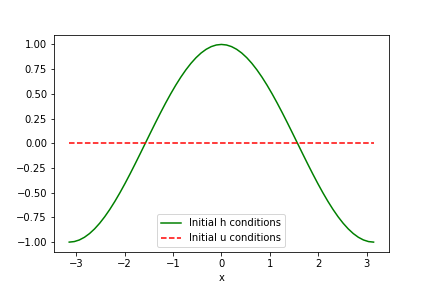
\includegraphics[width=\textwidth]{initial_condition_cos.png}
	\caption{\label{initialconditioncos}Initial condition such that $u$ is zero everywhere and $h$ is $\cos(x)$}
\end{minipage}
	\begin{minipage}{.5\textwidth}
	\ContinuedFloat
	%\centering
	\captionsetup{width=0.9\textwidth}
	\captionsetup{justification=centering}
	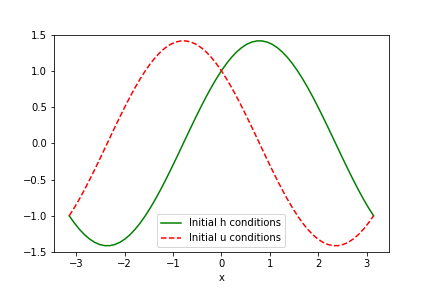
\includegraphics[width=\textwidth]{initial_condition_cossin.png}
	\caption{\label{initialconditioncossin}Initial condition such that $u$ is $\cos(x) - \sin(x)$ and $h$ is $\cos(x) + \sin(x)$}
\end{minipage}
\end{figure}

To begin with, we will compare the results of our numerical schemes to the analytic solution.
We start with the initial condition 
\begin{eqnarray}
u  & =  & 0 \\
h & = &  \cos(x)
\end{eqnarray}
shown in Figure \ref{initialconditioncos} for which it is possible to find an analytic solution of the shallow water equations:
\begin{equation}\label{uanalytic}
u = \sin(x)\sin(t)
\end{equation}
\begin{equation}\label{hanalytic}
h = \cos(x)\cos(t).
\end{equation}
If we choose the interval $[-\pi, \pi]$ then these solutions are periodic.

To carry out this test, we have used $c = 0.1$, $nx = 60$, $nt = 60$ and the domain $=\pi\leq x \leq \pi$.
\renewcommand\theContinuedFloat{\alph{ContinuedFloat}}
\begin{figure} [H]
	\begin{minipage}{.5\textwidth}
		\ContinuedFloat*
		%\centering
		\captionsetup{width=0.9\textwidth}
		\captionsetup{justification=centering}
		\includegraphics[width=\textwidth]{comparison_with_analytic_u.png}
		\caption{\label{exact velocity} Velocity, $u$, for the initial condition shown in Figure \ref{initialconditioncos}. } 
	\end{minipage}
	\begin{minipage}{.5\textwidth}
		\ContinuedFloat
		%\centering
		\captionsetup{width=0.9\textwidth}
		\captionsetup{justification=centering}
		\includegraphics[width=\textwidth]{comparison_with_analytic_h.png}
		\caption{\label{exact height} Height, $h$, for the initial condition shown in Figure \ref{initialconditioncos}.} 
	\end{minipage}
\end{figure}
Figures \ref{exact velocity} and \ref{exact height} show that for the smooth initial condition $u= 0$ and $h= \cos(x)$, all the numerical schemes approximate very closely to the analytical solution. 

%Therefore we calculae the L2 error norms of the schemes in Table \ref{errortable}. These show that the staggered semi-implicit method is the most accurate for both $u$ and $h$, as expected as it is second order in time and space whereas the other schemes are first order in time and second order in space. The co-located implicit scheme is more inaccurate than the other schemes for $u$. This may be because of cumulative errors when inverting and multiplying the matrix used in the scheme.

%\begin{table}[H]
%	\centering
%	\begin{tabular}{|c | c| c|} 
%		\hline
%		\textbf{Numerical Scheme} & \textbf{Error in u} & \textbf{Error in h}  \\
%		\hline
%		Co-located Explicit & $5.6 \times 10^{-6}$ & $2.3 \times 10^{-4}$\\ 
%		\hline
%		Staggered Explicit &  $1.5 \times 10^{-6}$ & $2.3 \times 10^{-4}$\\
%		\hline
%		Co-located  Implicit & $2.0 \times 10^{-4}$ & $1.9 \times 10^{-4}$ \\
%		\hline
%		Staggered Semi-implicit & $1.4 \times 10^{-6}$ & $7.7\times 10 ^{-7}$ \\
%	\hline
%	\end{tabular}
%	\caption{Error L2 norms for all 4 numerical schemes}
%	\label{errortable}
%\end{table}

If we take the initial condition 
\begin{eqnarray} \label{ic}
u  =  \cos(x) - \sin(x)\\
 h  =  \cos(x) + \sin(x)
\end{eqnarray}
shown in Figure \ref{initialconditioncossin} for we can also find an analytic solution of the shallow water equations:
\begin{eqnarray} \label{as}
u = (\cos(x) - \sin(x))(\cos(t) - \sin(t))\\
h = (\cos(x) + \sin(x))(\cos(t) + \sin(t))
\end{eqnarray}
Again we choose the interval $[-\pi, \pi]$ so that these solutions are periodic.
We would like to see if the orders of accuracy with respect to $\Delta x$ and $\Delta t$ found by Taylor expansion analysis in section \ref{numericalmethodssection} are correct, by using this initial condition and analytic solution.

For a fixed Courant number and fixed $x$ domain and total time, if we vary $\Delta x$, we vary $\Delta t$ too. Therefore plotting the error against $\Delta x$ or against $\Delta t$ gives the same result.  

To find the order of the error with respect to $\Delta t$, we use a large courant number of $c = 0.5$ as $c \propto \frac{\Delta t}{\Delta x}$ so for large courant numbers $\Delta t$ dominates. We find the error of the solution at time $\frac{\pi}{12}$ for $nx = [120, 240, 360, 480]$ and $nt = [10, 20, 30, 40]$ on the domain $-\pi \leq x \leq \pi$. The results of this test are displayed in Figure \ref{uerrorcossindt} and Figure \ref{herrorcossindt}.

To find the order of the error with respect to $\Delta x$, we repeat this process but use a small courant number of $c = 0.005$ as $c \propto \frac{\Delta t}{\Delta x}$ so for small courant numbers $\Delta x$ dominates. We find the error of the solution at time $\pi$ for $nx = [12, 24, 36, 48]$ and $nt = [1200, 2400, 3600, 4800]$ on the domain $-\pi \leq x \leq \pi$. The results of this test are displayed in Figure \ref{uerrorcossindx} and Figure \ref{herrorcossindx}.

\begin{figure} [H]
	\begin{minipage}{.5\textwidth}
		\ContinuedFloat*
		%\centering
		\captionsetup{width=0.9\textwidth}
		\captionsetup{justification=centering}
		\includegraphics[width=\textwidth]{{uerror_compared_dt_cossin_c=0.5}.png}
		\caption{\label{uerrorcossindt}Log plot for the solution error of $u$ vs $\Delta t$ where $c = 0.1$. Lines proportional to $\Delta t$ and $\Delta t^{2}$ are plotted for reference.} 
	\end{minipage}
	\begin{minipage}{.5\textwidth}
		\ContinuedFloat
		%\centering
		\captionsetup{width=0.9\textwidth}
		\captionsetup{justification=centering}
		\includegraphics[width=\textwidth]{{herror_compared_dt_cossin_c=0.5}.png}
		\caption{\label{herrorcossindt}Log plot for the solution error of $h$ vs $\Delta t$ where $c= 0.1$. Lines proportional to $\Delta t$ and $\Delta t^{2}$ are plotted for reference.} 
	\end{minipage}
\end{figure}

\begin{figure}[H]
	\begin{minipage}{.5\textwidth}
		\ContinuedFloat*
		%\centering
		\captionsetup{width=0.9\textwidth}
		\captionsetup{justification=centering}
		\includegraphics[width=\textwidth]{{uerror_compared_dx_cossin_c=0.005}.png}
		\caption{\label{uerrorcossindx}Log plot for the solution error of $u$ vs $\Delta x$ where $c=0.005$. Lines proportional to $\Delta x^{2}$ are plotted for reference.} 
	\end{minipage}
	\begin{minipage}{.5\textwidth}
		\ContinuedFloat
		%\centering
		\captionsetup{width=0.9\textwidth}
		\captionsetup{justification=centering}
		\includegraphics[width=\textwidth]{{herror_compared_dx_cossin_c=0.005}.png}
		\caption{\label{herrorcossindx}Log plot for the solution error of $h$ vs $\Delta x$ where $c = 0.005$. Lines proportional to $\Delta x^{2}$ are plotted for reference.} 
	\end{minipage}
\end{figure}

The gradients of the lines plotted in Figures \ref{uerrorcossindt} - \ref{herrorcossindx}  are in Table \ref{gradientdt} and Table \ref{gradientdx}. These gradients are found by using python's least square polynomial fit function on the log relationships between the error and $\Delta x$ and the error and $\Delta t$ (choosing the polynomial to be order one). 

Our results agree closely with the order of accuracy calculated by the taylor expansion apart from the time order of accuracy in the staggered explicit case. This may be because the scheme may already be exhibiting instabilities (as it become unstable at $c = 1$.)

Now we would like to test some of the numerical properties of the schemes.

\begin{table}[H]
	\centering
	\begin{tabular}{|c | c| c| c|} 
		\hline
		\textbf{Numerical Scheme}  & $u$ error vs $\Delta t$ & $h$ error vs $\Delta t$ & Order in time \\
		\hline
		Co-located Explicit & 1.02 & 1.01 & 1\\ 
		\hline
		Staggered Explicit & 0.13 & 0.02 & 1\\
		\hline
		Co-located Implicit & 0.95 & 1.01 & 1\\
		\hline
		Staggered Implicit & 2.00 & 2.00 & 2\\
		\hline
	\end{tabular}
	\caption{Time order of accuracy from numerical schemes taken from Figures \ref{uerrorcossindt} - \ref{herrorcossindt} compared to spatial order of accuracy from Taylor expansion}
	\label{gradientdt}
\end{table}

\begin{table}[H]
	\centering
	\begin{tabular}{|c | c| c| c|} 
		\hline
		\textbf{Numerical Scheme} & $u$ error vs $\Delta x$ &  $h$ error vs $\Delta x$ & Order in space\\
		\hline
		Co-located Explicit & 1.94 & 2.03 & 2 \\ 
		\hline
		Staggered Explicit & 1.93 & 1.99 & 2 \\
		\hline
		Co-located Implicit & 2.00 & 1.97 & 2 \\
		\hline
		Staggered Implicit & 1.99 & 2.01 & 2 \\
		\hline
	\end{tabular}
	\caption{Spatial order of accuracy from numerical schemes taken from Figures \ref{uerrorcossindx} - \ref{herrorcossindx} compared to spatial order of accuracy from Taylor expansion}
	\label{gradientdx}
\end{table}


\subsection{Test 1}
We found using Von-Neumann stability analysis that the co-located explicit scheme is unstable for Courant numbers higher than 2, but that the co-located implicit scheme is unconditionally stable (ie. stable for all Courant numbers). To test this we ran both schemes using a range of Courant numbers with the initial condition $h = \cos(x) + \sin(x)$ and $u = \cos(x) -\sin(x)$ (shown in Figure \ref{initialconditioncossin}) and $nx = 100$ and $nt = 100$.

Figures \ref{velocity_varying_courant} and \ref{height_varying_courant} show for Courant numbers larger than $2$ the co-located explicit method is unstable for both $u$ and $h$. By contrast, for large Courant numbers, the co-located implicit method remains stable for both $u$ and $h$. This is as expected from the Von-Neumann stability analysis.

\begin{figure}[H]
	\begin{minipage}{.5\textwidth}
		\ContinuedFloat*
		%\centering
		\captionsetup{width=0.9\textwidth}
		\captionsetup{justification=centering}
		\includegraphics[width=\textwidth]{velocity_varying_courant.png}
		\caption{\label{velocity_varying_courant} Velocity for varying Courant numbers for the co-located explicit and implicit methods} 
	\end{minipage}
	\begin{minipage}{.5\textwidth}
	\ContinuedFloat
	%\centering
	\captionsetup{width=0.9\textwidth}
	\captionsetup{justification=centering}
	\includegraphics[width=\textwidth]{height_varying_courant.png}
	\caption{\label{height_varying_courant} Height for varying Courant numbers for the co-located explicit and implicit methods} 
\end{minipage}
\end{figure}

\subsection{Test 2}
\begin{figure}[H]
\begin{center}
\begin{minipage}{.5\textwidth}
	\centering
	\captionsetup{width=2\textwidth}
	\captionsetup{justification=centering}
	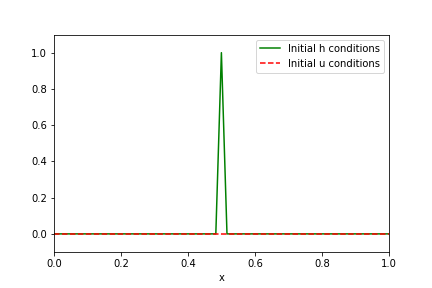
\includegraphics[width=\textwidth]{initial_condition_spike.png}
	\caption{\label{initialconditionspike}Initial condition such that $u$ is zero everywhere and $h$ is zero everywhere apart from one point at the centre where it is one} 
\end{minipage}
\end{center}
\end{figure}

When looking at the dispersion relation for the co-located grid it seems that the results produced by the scheme may be unphysical. By contrast we expect the staggered grid to produce more physical results. We test this hypothesis by taking the different less smooth initial condition that $u =0$ and $h = 0$ apart from one point in the centre where it is $1$ (shown in Figure \ref{initialconditionspike}) and plotting the solutions of $u$ and $h$ at multiple time steps for the co-located explicit scheme and the staggered explicit scheme.

For this test we have used $nx = 20$ and $nt = 10$ on the $x$ domain $0 \leq x \leq 1$ and a Courant number of $0.1$.

\begin{figure} [H]
	\begin{center}
	\begin{minipage}{.6\textwidth}
		\ContinuedFloat*
		%\centering
		\captionsetup{width=1.5\textwidth}
		\captionsetup{justification=centering}
		\includegraphics[width=\textwidth]{velocity_spike.png}
		\caption{\label{velocity_spike} Velocity at different timesteps using the co-located explicit method and the staggered explicit method} 
	\end{minipage}
\end{center}
\end{figure}
\begin{figure}[H]
	\begin{center}
	\begin{minipage}{.6\textwidth}
		\ContinuedFloat
		%\centering
		\captionsetup{width=1.5\textwidth}
		\captionsetup{justification=centering}
		\includegraphics[width=\textwidth]{height_spike.png}
		\caption{\label{height_spike} Height at different timesteps using the co-located explicit method and the staggered explicit method} 
	\end{minipage}
\end{center}
\end{figure}

As expected the results shown in Figures \ref{velocity_spike} and \ref{height_spike} for the co-located grid are unphysical. The fluid does spread out but it does not go to the next meshpoint, instead skipping this meshpoint out and moving to the next meshpoint along. In Figure \ref{height_spike} we see that the two points around the central grid point (hereafter referred to as $x_{m}$) never have any height for the co-located grid so the fluid passes from $x_{m}$ to $x_{m-2}$ and $x_{m+ 2}$ without passing through $x_{m-1}$ and $x_{m+1}$ which is clearly unphysical. Similarly in Figure \ref{velocity_spike} there is never any velocity at the gridpoints $x_{m-2}$ and $x_{m+2}$ for the co-located grid which is again unphysical. 

In contrast, the staggered scheme produces physically realistic results for this initial condition. Figure \ref{height_spike} shows that the height spreads out evenly using all grid points. Figure \ref{velocity_spike} shows further that the velocity is non-zero at the gridpoints where the wave has propagated as expected from a physical system.


\subsection{Test 3}
Finally we compare the computational cost of the four schemes, by comparing the time it takes for each scheme to run, starting from the initial condition $u = \cos(x) - \sin(x)$ and $h = \cos(x) + \sin(x)$ (shown in Figure \ref{initialconditioncossin}) on an $x$-domain of $-\pi \leq x \leq \pi$, with Courant number $0.1$ and with the same number of time steps ($nt = 1000$) and space steps ($nx = 1000$).

\begin{table}[H]
	\centering
	\begin{tabular}{|c | c|} 
		\hline
		\textbf{Numerical Scheme} & \textbf{Time (3sf)}  \\
		\hline
		Co-located Explicit & 1.90 s \\ 
		\hline
		Staggered Explicit & 1.69 s \\
		\hline
		Co-located  Implicit & 3.45 s \\
		\hline
		Staggered Implicit & 5.41 s \\
		\hline
	\end{tabular}
	\caption{Time taken for each numerical scheme to run for the initial condition that $u$ is $\cos(x) - \sin(x)$ and $h$ is $\cos(x) + \sin(x)$.}
	\label{timingtable}
\end{table}


The co-located explicit and staggered explicit schemes take a similar amount of time as expected as they have the same number of floating point operations per iteration.

The implicit schemes have a higher computational cost than the explicit schemes as they involve one inversion of a matrix (O($n^{3}$) floating point operations for an $n \times n$ matrix) and at each iteration to find $u^{m}$ or $h^{m}$ a matrix-vector multiplication (O($n^{2}$) floating point operations for an $n \times n$ matrix). Therefore as expected the implicit schemes take longer than the explicit schemes.

The staggered implicit scheme has the highest computational cost, as constructing $b_{i}$ in the $A_{ij}x_{j} = b_{i}$ matrix equation involves nine floating point operations compared to three floating point operations to construct $b_{i}$ in the co-located implicit scheme. Therefore it takes the longest of the four schemes.  

\section{Conclusions}

From the results listed in Section \ref{resultssection}, we can conclude the following:

\begin{itemize}
	\item The implicit staggered method is the most accurate of the 4 schemes
	\item When working with high Courant numbers (e.g. if the meshgrid spacing is very fine so $\Delta x$ is small or if $H$ or $\Delta t$ are very large), it is better to choose implicit methods as they are stable for all Courant numbers whereas explicit methods can have large instabilities (from Test 1)
	\item Staggered grids produce more physically realistic results than co-located grids for certain initial conditions (from Test 2)
	\item When working with small Courant numbers, it is better to choose explicit methods as they are less computationally expensive than implicit methods (from Test 3)
\end{itemize}


\begin{thebibliography}{9}
	\addcontentsline{toc}{part}{Bibliography}
	\bibitem{MPE textbook}
	Cotter, C. and Weller, H., (2018), \textquoteleft Numerical Methods\textquoteright, Ch.5 in Crisan, D (eds.), \textit{Mathematics of Planet Earth: a primer}, World Scientific Publishing Europe Ltd., London.
	\bibitem{implicit}
	Casulli, V. and Cattani, E., (1994), \textquoteleft Stability, Accuracy and Efficiency of a Semi-Implicit Method for Three-Dimensional Shallow Water Flow\textquoteright, \textit{Computers Math. Applic}, \textbf{27(4)}, 99-112.
\end{thebibliography}
\end{document}